\documentclass[/home/greg/Thesis/main/main.tex]{subfiles}

\begin{document}
\graphicspath{{/home/greg/Neutron_star_modelling/SpindownRate/img/}}

\section{Physical observables: spin-down rate $\dot{\nu}$}

The second observable which is often considered in characterising periodic
patterns in pulsar signals is the slowdown rate. In this simple model the
slowdown rate is given by $\ddot{\Phi}$, however calculating an analytic
expression from \eqref{eqn: Phi_dot} is difficult, although possible. As an alternative, we
can use the method proposed by \citet{Lyne2010} to measure changes in the
spindown of observed pulsars. Second order Taylor expansions are fitted to
short sections of data of length $T$ and the resulting coefficient $\dot{\nu}$
is recorded. Repeating this process every $\sim T/4$ through the data set
builds picture of how the spindown varies with time. We choose $T$ such that it
is a fraction of the precession period over which we expect quantities to be
modulated.

\subsection{Spin-down variations due to free-precession}
Without an EM torque, the average spin-down rate should be zero. However, if
the body undergoes free precession, this will produce periodic variations. The
magnitude of these can be calculated by differentiating equation (49) from 
\citet{Jones2001} twice to give
\begin{equation}
    \Delta\ddot{\Phi}_{\mathrm{FP}} =\dot{\psi}^{2} \theta \cot\chi. 
    \label{eqn: spin-down variations FP}
\end{equation}


\begin{figure}[ht]
\centering
	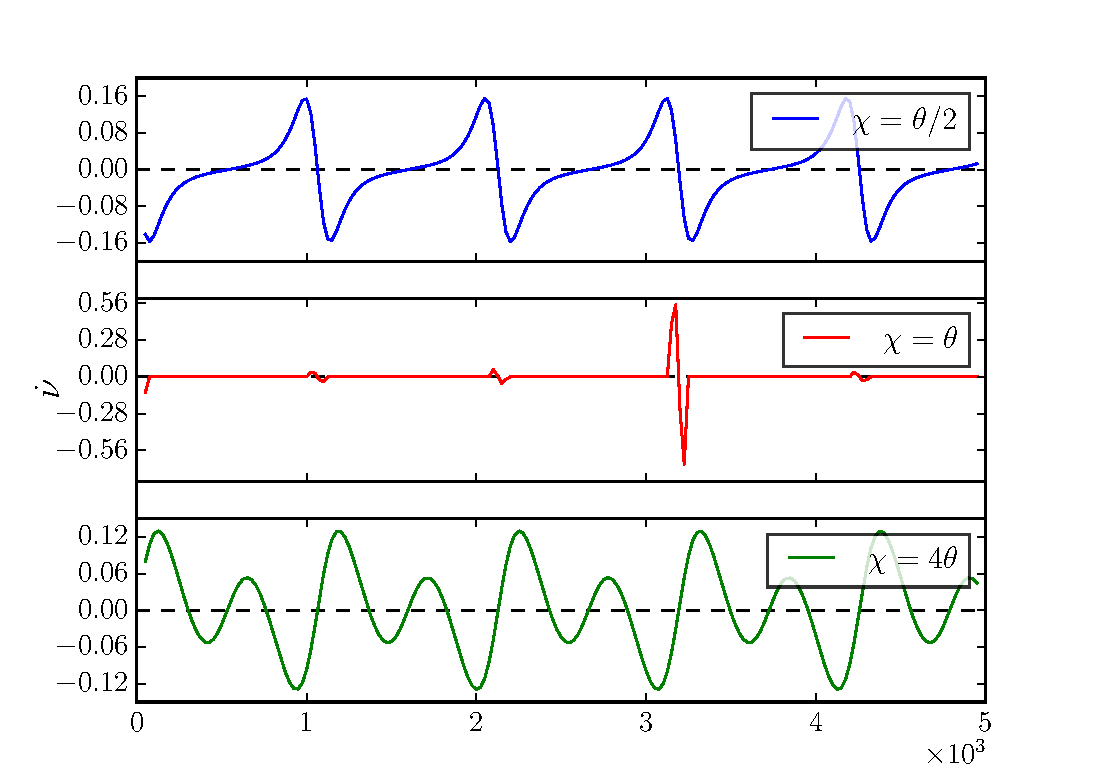
\includegraphics[width=0.5\textwidth]{nu_dot_no_torque.pdf}
\caption{Slow down rate }
\label{fig: nu_dot no torque}
\end{figure}

The variations seen in figure \ref{fig: nu_dot no torque} are the result of
free precession. As there is no torque, the overall spindown is zero. However,
due to precession the magnetic dipole performs a slow rotation about the
deformation axis. During half the cycle it counter-rotates and in the other
half it corotates with the rapid rotation about the angular momentum vector.
The result is a symmetric modulation of the spindown about zero with magnitude
given by equation \eqref{eqn: spin-down variations FP}.

\subsection{Spin-down due to EM torque}
When we include the EM torque we will have a non-zero average spin-down rate. 
We can measure this directly from equation \eqref{eqn: surface magnetic field}:
rearranging for $\dot{\Omega}$ we have
\begin{equation}
    \dot{\Omega} = -\frac{B_{0}^{2}R^{6} \sin^{2}\alpha \Omega^{3}}{6I_{0}c^{3}},
\end{equation}
writen in terms of the model parameters this is
\begin{equation}
\dot{\nu} = -\frac{1}{3\pi}\frac{R \Omega^{3}}{c} \sin^{2}\alpha \epsA
\end{equation}
In general the spin-down is approximately constant over a given observation
time. As a result we estimate the spin-down rate by the initial value:
\begin{equation}
    \dot{\nu}_{0} = -\frac{1}{3\pi}\frac{R \Omega_{0}^{3}}{c} \sin^{2}\alpha \epsA
    \label{eqn: spin-down initial EM}
\end{equation}
In general we can approximate $\alpha\approx\chi$ to get a handle for the 
magnitude of $\dot{nu}_{0}$.

In figure \ref{fig: nu_dot with torque} we plot a typical spin-down calculation
showing the non-zero average spin-down due to EM torque along with the 
variations due to precession.
\begin{figure}[ht]
\centering
	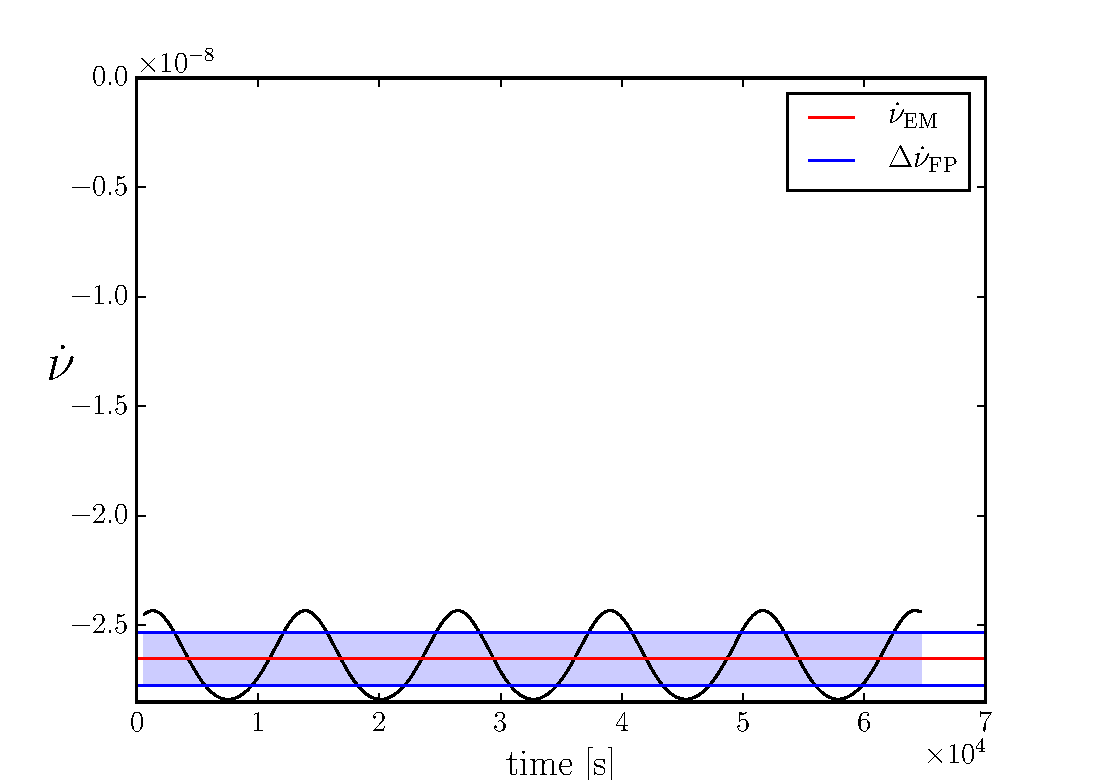
\includegraphics[width=0.5\textwidth]{nu_dot_with_torque.pdf}
\caption{Spin-down rate when including the EM torque}
\label{fig: nu_dot with torque}
\end{figure}


%\subsubsection{Pulse amplitude}
%Assuming a fixed magnitude of the magnetic dipole, the pulse amplitude will 
%depend on the orientation of the magnetic dipole to the observer. It will be 
%maximal when pointing directly at the observer and presumably fall off as the
%angle between the two grows. To model this we take an observers position as 
%$\Phi_{O}, \Theta_{O}$ and then assume the emission region follows
%a two dimensional Gaussian:
%\begin{equation}
%A(\Phi, \Theta) = A_{0} \textrm{exp} \left(
%                         -\frac{\tilde{\Phi}^{2}}{2\sigma_{\Phi}^{2}}
%                         -\frac{\tilde{\Theta}^{2}}{2\sigma_{\Theta}^{2}}
%                                     \right)
%\label{eqn: Amplitude}
%\end{equation}•
%where $\tilde{\Phi}=\mod_{2\pi}(\Phi)-\Phi_{O}$ and 
%$\tilde{\Theta}=\mod_{\pi}(\Theta) - \Theta_{O}$. Computing the angles $\Phi$ and $\Theta$ from numerical
%solutions of the original ODEs and using the above emission model gives 
%the pulse amplitude as seen be an observer. An example of a solution showing
%the individual pulses along with the modulation due to free precession is
%given in figure \ref{fig: amplitude_variation}
%\begin{figure}[htb]
%\centering
%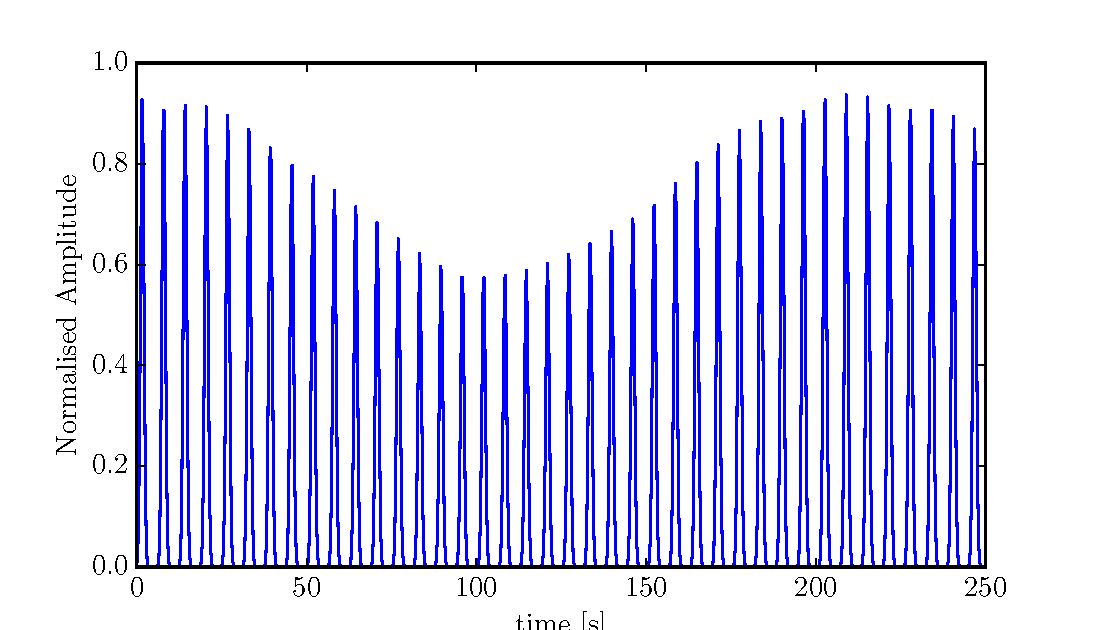
\includegraphics[width=.75\textwidth]{amplitude_variation}
%\caption{Amplitude variation using a 2D Gaussian emission.}
%\label{fig: amplitude_variation}
%\end{figure}•

%\FloatBarrier
%\subsubsection{Pulse width}
%The modulation of the amplitude coincides with modulations of the pulse width.
%These have been measured with great accuracy by \citet{Lyne2010} and their
%correlation with perceived changes in the spindown is key evidence for the two
%state switching model. We can extract the pulse width analytically from
%equation \eqref{eqn: Amplitude} by noting that $\Theta$ varies on the slow
%precession timescale while $\Phi$ varies on the rapid spin timescale. We are
%looking to measure the variations with respect to the slow precession timescale
%so we can treat it as a constant. The full with at half maximum, corresponding
%to the $W_{50}$ value of \citet{Lyne2010} occurs when
%\begin{align}
%A(\Phi, \Theta) = A_{0} \frac{1}{2} 
%\end{align}
%The condition for a full width half maximum at a fixed value of $\tilde{\Theta}$ 
%is then
%\begin{align}
%\tilde{\Phi}_{50} = \pm\sigma_{\Phi}\left(\ln(2) 
%          - \frac{\tilde{\Theta}}{\sigma_{\Theta}^{2}}\right)^{1/2}
%\end{align}
%If $P$ is the period of the rapid spin motion, then the fraction $W_{50}/P$
%must be equal the fraction of the cycle spent above the full width half maximum
%which is given by $2\tilde{\Phi}_{50} / 2\pi$. Writing this in terms of the
%frequency $\dot{\Phi}$ rather than period we have
%\begin{equation}
%W_{50} = \frac{1}{\pi\dot\Phi}\sigma_{\Phi}\left(\ln(2) 
%     - \frac{\tilde{\Theta}}{\sigma_{\Theta}^{2}}\right)^{1/2}
%\label{eqn: pulse width}
%\end{equation}•
%
%In figure \ref{fig: PulseWidthModulation} we plot the pulse width as a function
%of time for a canonical pulsar with $\chi=70^{\deg}$. 
%\begin{figure}[ht]
%\centering
%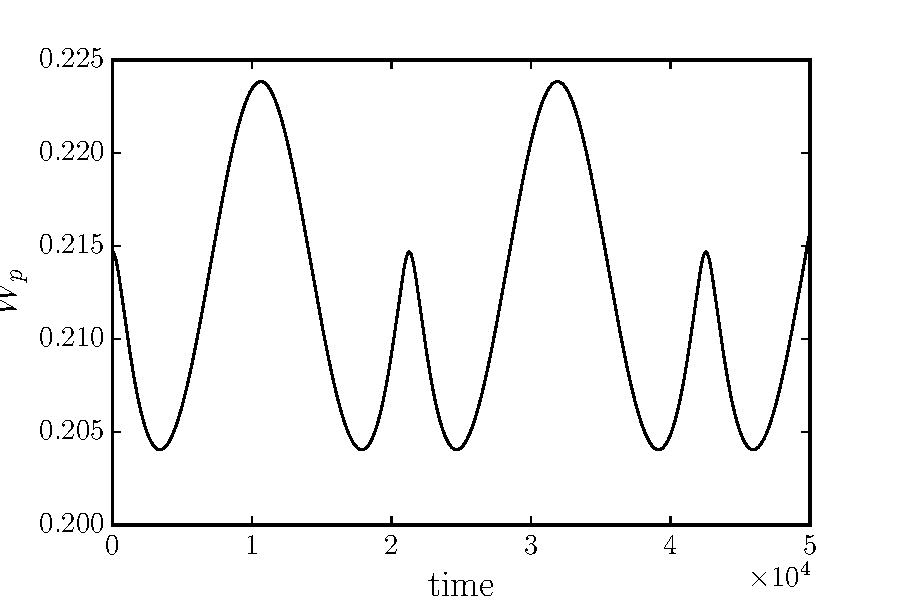
\includegraphics[width=.5\textwidth]{Pulse_width_modulation}
%\caption{Pulse width as calculated by equation \eqref{eqn: pulse width} }
%\label{fig: PulseWidthModulation}
%\end{figure}•
%
%\FloatBarrier

%\biblio
\end{document}

